\chapter{Modèle d'architecture CxSOM}
\graphicspath{{02-SOM/}}
\minitoc

En réponse à la problématique de construire des architectures décentralisées de cartes de Kohonen, nous proposons dans cette thèse une version légèrement modifiée de carte auto-organisatrices, CxSOM. L'algorithme classique est modifié pour permettre à une carte de prendre plusieurs entrées; la recherche du BMU est également transformée.
Nous présentons dans cette partie l'algorithme CxSOM et les paramètres utilisés.

\section{Carte de Kohonen standard}
L'algorithme CxSOM est directement dérivé de l'algorithme d'une carte de Kohonen classique. Le principe général d'une carte de Kohonen a été décrit dans le chapitre précédent; nous définissons ici plus précisément le modèle et les équations qui serviront de base pour la définition de l'algorithme CxSOM.

\subsection{Algorithme et notations}
Une carte de Kohonen est un graphe, généralement une ligne 1D ou une grille 2D de $N$ noeuds. Nous utiliserons principalement dans cette thèse des cartes en une et deux dimensions, c'est à dire des lignes et des grilles. Les notations présentées ici sont valables pour des cartes de dimension quelconque.

L'algorithme et les notations sont résumés en figure~\ref{fig:one_map_not}
Les entrées sont notées $\inpx$, tirées dans un espace d'entrée $D$. Le poids associé à un noeud est noté $\w_e \in D$. Sa \emph{position} dans la carte est indexée par $p$. Dans toute cette thèse, les positions seront indexées entre $0$ et $1$. L'ensemble des poids est noté ${\w_e(p), p \in [0,1]}$.
Une étape $t$ de l'algorithme de mise à jour d'une carte de Kohonen est le suivant:
\begin{enumerate}
\item\label{enum:inp} Une entrée $\inpx_t$ est présentée à la carte.
\item\label{enum:act} Une \emph{activité} $a_e(\inpx_t,p)$ est calculée dans la carte. Cette étape est déjà une légère modification souvent utilisée de l'algorithme de Kohonen. On cherche alors l'index du maximum de l'activité au lieu du minimum des distances.
\item L'unité ayant l'activité maximale est la \emph{Best Matching Unit} de la carte. Sa position est notée $\bmu$.
\item Chaque poids $\w_e$ est déplacé vers l'entrées $\inpx$, en fonction de sa distance dans la carte à la best matching unit : 
\begin{equation}
\w_e(p,t+1) = \w_e(p,t) + \alpha h(\bmu,p)(\inpx_t - \w_e(p,t))
\label{eq:update}
\end{equation}
\end{enumerate}

$h(\bmu,p)$ est la \emph{fonction de voisinage}. Elle est maximale en $p = \bmu$ et décroissante autour de cette position. Dans notre étude, les fonctions de voisinage sont triangulaires, donc maximales en $\bmu$, décroissante sur le rayon de voisinage $h_e$ et nulle après.
La fonction d'activité présente à l'étape \ref{enum:act} est une activation gaussienne:
\begin{equation}\label{eq:act}
a_e(\inpx_t,p) = \exp{\frac{\lVert \inpx_t-\w\ext(p) \rVert ^2}{2\sigma^2}}
\end{equation}

\begin{figure}
\centering
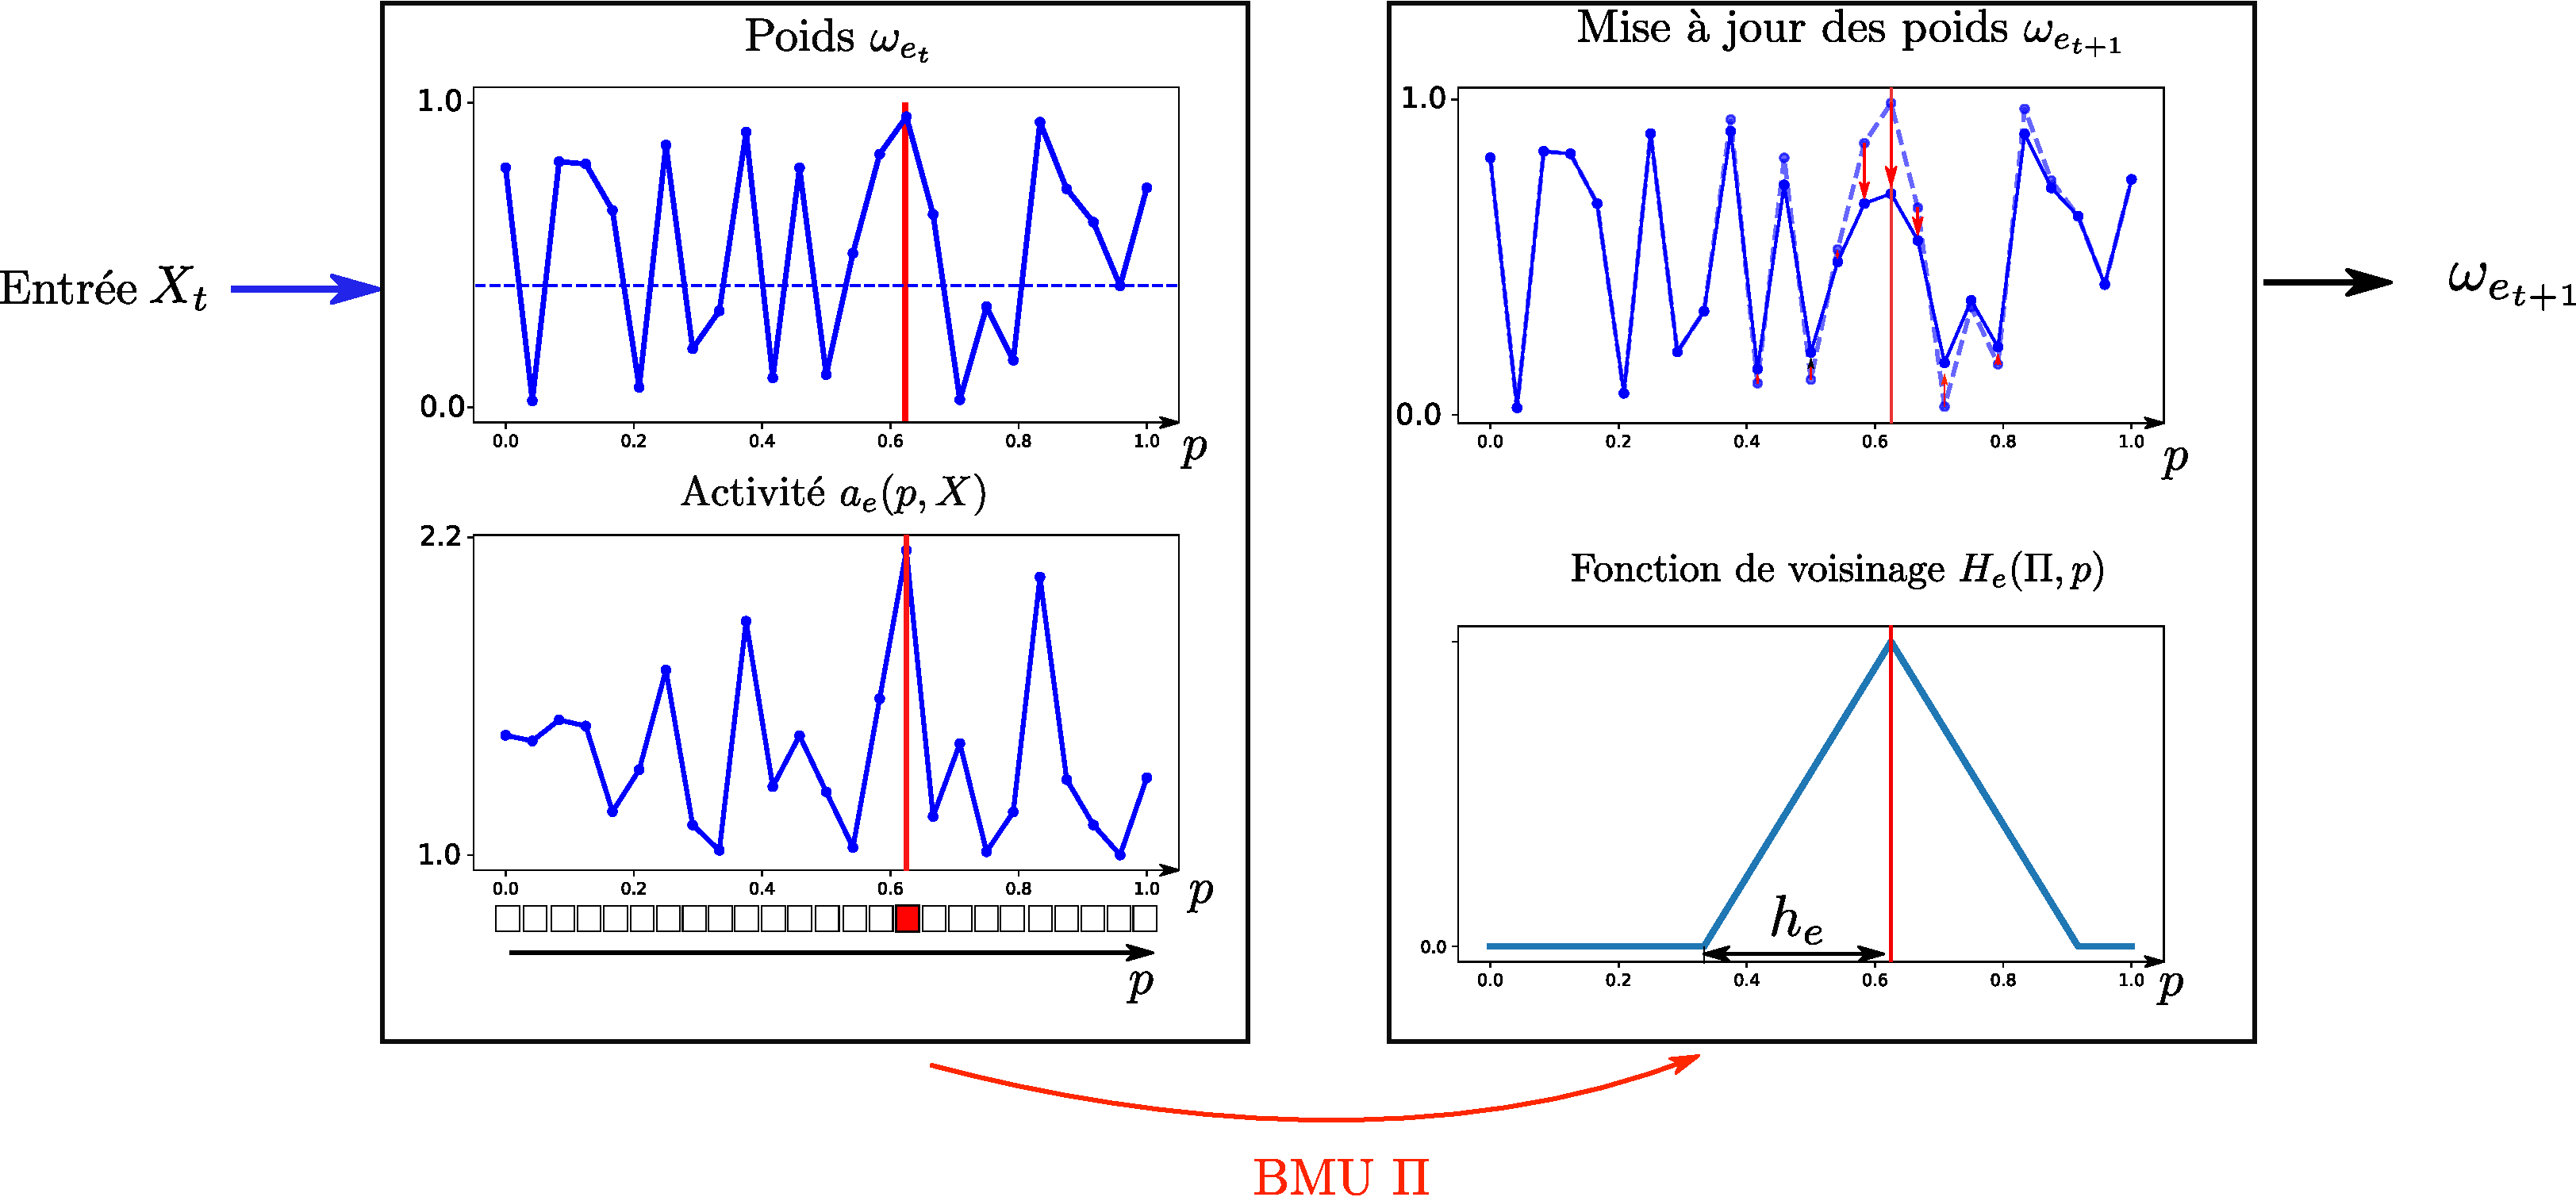
\includegraphics[width=\textwidth]{one_map_one_layer2.pdf}
\caption{Notations utilisées dans une carte de Kohonen simple}
\label{fig:one_map_not}
\end{figure}

\subsection{Paramètrage d'une carte de Kohonen}
\subsubsection{Nombre de neurones d'une carte}
Le nombre de neurones d'une carte définit le niveau de quantification qu'on souhaite effectuer. Pour des opérations de classification, on choisira un nombre de neurones plus élevé que le nombre de classes, afin de pouvoir avoir plusieurs prototypes par classe.
Dans cette thèse, nous utilisons des cartes 1D comportant 500 noeuds. Le nombre de noeud est assez élevé pour pouvoir bien cartographier des ensembles de plus grande dimension. Ce nombre de noeud est proche de ce qu'on peut trouver dans la littérature; les cartes ont souvent entre 500 et 1000 noeuds.  

\subsubsection{Taux d'apprentissage $\alpha$}

Le taux d'apprentissage $\alpha$ détermine la proportion dans laquelle chaque poids est déplacé vers l'entrée lors de sa mise à jour. Dans l'algorithme standard, le taux d'apprentissage décroit au cours de l'apprentissage. Au début de l'apprentissage, $\alpha$ est élevé, ce qui assure une organisation "grossière" rapide de la carte. $\alpha$ diminue ensuite de manière à cartographier plus localement les données. Cette décroissance assure principalement la convergence des poids de la carte au cours de l'apprentissage.
Dans l'algorithme CxSOM, nous utiliserons un taux d'apprentissage constant au cours de l'apprentissage. L'organisation des poids sera initialement un peu plus lente qu'une carte classique, mais cela permet de garder les paramètres constant au cours de l'apprentissage.
\comment{on n'aime pas les valeurs qui dépendent de $t$}.
Nous observerons qu'en choisissant les bons paramètres, la convergence de la carte s'effectue correctement.

\subsubsection{Topologie de la carte}
Les choix concernent la forme du graphe servant de structure à la carte : grille 1D, 2D, arbre. Ces éléments ont été décrits en section [ref].
Le choix de la fonction de voisinage est déterminant dans la topologie de la carte, et en particulier le rayon de voisinage $h_e$ qui détermine l'elasticité de la carte.
Cette valeur détermine quelles unités voisines du BMU seront affectées par le déplacement du BMU.
Plus le rayon $h_e$ est grand, plus la partie de la carte déplacée vers l'entrée lors de la mise à jour est étendue. Un grand rayon d'apprentissage permet un dépliement plus rapide de la carte de Kohonen, mais l'apprentissage est peu précis. Les données apprises alors rapidement oubliées par le déplacement des poids.
Un petit rayon d'apprentissage permet de déplacer les poids concentrés dans une petite région sans affecter toute la carte. Cela permet donc d'apprendre de nouvelles entrées sans oublier les parties déjà apprises. Par contre, utiliser un petit rayon de voisinage au début de l'apprentissage empêche une carte de bien se déplier et d'apprendre une structure globale des données. On doit donc trouver un compromis entre apprentissage de nouvelles données et mémoire des données déjà apprises.
Dans l'algorithme classique, ce compromis est trouvé en faisant décroitre le rayon de voisinage au cours de l'apprentissage. Un grand rayon de voisinage permet à la carte de se déplier rapidement en apprenant une structure globale des données. Sa décroissance permet d'affiner l'apprentissage des données à un niveau plus fin. 
Dans l'algorithme CxSOM, nous utiliserons un rayon de voisinage constant.

\section{Modèle CxSOM}

Le but de cette thèse est de proposer un modèle permettant d'associer des cartes auto-organisatrices dans n'importe quel type d'architecture. En particulier, on cherchera à construire des architectures non-hiérarchiques de cartes, par exemple en figure~\ref{fig:archi_non_hierarchique}.

\begin{figure}
\centering
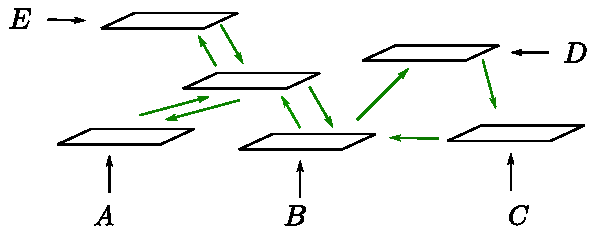
\includegraphics[width=0.6\textwidth]{architecture.pdf}
\caption{Exemple d'architecture modulaire \emph{non-hiérarchique} de cartes de Kohonen. Les entrées sont $A,B,C,D,E$ quelconques. Chaque carte peut ou non prendre une entrée ; les connexions sont réciproques ou non.}
\label{fig:archi_non_hierarchique}
\end{figure}

Dans ce modèle, l'algorithme original de Kohonen est modifié afin de connecter des cartes entre elles, et d'autoriser des connexions non-hiérarchiques.
La connexion entre une carte A et une carte B est réalisée lorsque la carte B prend comme entrée la position du Best Matching Unit de A. 
Considérons G, le graphe de connexions des cartes. Ce graphe est \emph{orienté} et les \emph{boucles} sont autorisées. C'est ce qu'on appelera \emph{architecture non-hiérarchique} de cartes, par opposition à des architectures hiérarchiques dans lesquelles le BMU d'une carte A est donné en entrée d'une carte B de façon unidirectionnelle. 

Chaque carte aura ainsi plusieurs entrées : une entrée \emph{externes} dans un espace d'entrée, facultative, et $k$ entrées \emph{contextuelles} qui sont les positions des BMUs des cartes qui lui sont connectées. Par ailleurs, la recherche du BMU doit être modifiée par rapport à l'originale : les rétroactions entre les cartes sont autorisées, la position du BMU de la carte A va donc influencer la position du BMU de la carte B, lequel modifie à nouveau le BMU de la carte A, etc. 
Notre algorithme implémente donc deux modifications principales par rapport à l'algorithme d'apprentissage d'une carte de Kohonen classique: 
\begin{itemize}
\item Les cartes possèdent plusieurs entrées, externes et contextuelles; les entrées contextuelles sont les positions des BMUs d'autres cartes. Le calcul de l'activité est donc modifié afin de prendre en compte ces différentes couches d'entrées.
\item La recherche du BMU est modifiée afin de gérer les rétroactions entre cartes.
\end{itemize}

La description du modèle CxSOM est détaillée en figure~\ref{fig:one_map}, dans un cas ou une carte reçoit deux connexions, et l'algorithme explicité en~\ref{algo:cxsom}.


\subsection{Gestion des entrées externes et contextuelles}

A un pas d'apprentissage $t$, une carte $M$ reçoit en entrée une entrée \emph{externe} notée $\inpx_t$ et $K$ entrées \emph{contextuelles} notées $\inpc_{0t},\cdots,\inpc_{Kt}$, qui sont les positions des BMU $\bmu$ des cartes qui lui sont connectées. La carte possède donc $k+1$ couches de poids. $\w_e$ correspond à l'entrée externe et $\w_{c0}, \cdots, \w_{cK}$ aux entrées contextuelles. On calcule une activité séparément sur chaque couche de poids selon la formule suivante : 
\begin{equation}
\label{eq:activite}
a(p,x) = \exp(\frac{(\w(p)-x)^2}{2\sigma^2} \; x = \inpx_t\; \text{ou}\; \inpc_{kt}, \; \w = \w_e \;\text{ou}\; \w_{ck}
\end{equation}
Les activités contextuelles sont moyennées en une activité $a_c(p,\mathbf{\inpc}_t)$, avec $\mathbf{\inpc_t} = (\inpc_{0t}, \cdots, \inpc{Kt})$. 
Les activités externes et contextuelles sont enfin fusionnées en une activité globale:
\begin{equation}
\label{eq:global_act}
a_g(p,\inpx_t,\mathbf{\inpc_t}) = \sqrt{a_e(p,\inpx_t)(\beta a_e(p,\inpx_t) + (1-\beta) a_c(p, \mathbf{\inpc_t})}
\end{equation}

Une convolution est appliquée sur cette activité globale. Cela évite les effets de plateau. Seule l'activation globale est considérée lors du calcul du BMU par relaxation, décrit en partie suivante. 

\subsection{Calcul du BMU par relaxation}

Contrairement à une carte simple, on ne peut pas calculer tous les BMUs de l'architecture en prenant l'argmax de $a_g$ dans chaque carte. A cause des influences mutuelles entre cartes, calculer le BMU d'une des cartes modifie les entrées des autres cartes de l'architecture, et donc leur BMU. Cette recherche est donc réalisée par un processus dynamique que l'on appelera \emph{relaxation}, menant à un consensus entre cartes : on cherche le point, s'il existe, où chaque BMU maximise l'activité globale de chaque carte.

Le processus de relaxation est donc une boucle imbriquée dans un pas d'apprentissage de l'architecture, indexée par $\tau$. Notons $\bmu\m[i]$ la position du BMU de la carte $i$, et $\mathbf{\bmu} = (\bmu\m[0], \cdots , \bmu\m[n])$, avec $n$ le nombre de cartes de l'architecture.
Au début d'un pas d'apprentissage, chaque carte est nourrie avec une entrée externe $\inpx^i_t$, et les activités externes $a_e^i(\inpx^i_t,p)$ de chaque carte peuvent être calculées.
La recherche du BMU suit le processus de relaxation suivant : 
\begin{enumerate}
\item Dans chaque carte $i$, la position $\bmu^i$ est initialisée à $\argmax_p(a_e^i(\inpx^i_t,p)$. Les entrées contextuelles sont alors initialisées en prenant le BMU correspondant aux connexions de l'architecture.
\item Tant que toutes les positions $\bmu^i$ ne sont pas stables, 
	\begin{enumerate}
	\item Dans chaque carte $i$, calculer les activités contextuelles et globales, définissant ainsi $p^{\star i} = \argmax_p(a_g(p,\mathbf{\inpc^i},\inpx^i)$
	\item Déplacer $\bmu^i$ vers $p^{\star i}$ : $\bmu^i \leftarrow \bmu^i \pm \Delta$ si $\lvert \bmu^i - p^{\star i} \rvert \geq \Delta$, $\bmu^i \leftarrow p^{\star i}$ sinon
	\end{enumerate}
	
\item Le BMU de chaque carte est pris comme la valeur finale stable de ce processus dynamique. Cette valeur est utilisée pour les mise a jour des poids.
\end{enumerate}

Il peut arriver que les positions se stabilisent sur un cycle limite. Dans ce cas, on arrêtera la relaxation arbitrairement; ce phénomène étant ponctuel, il n'influence pas l'apprentissage. Les paramètres des cartes de l'architecture sont choisis pour éviter de telles situations.

\begin{figure}
\centering
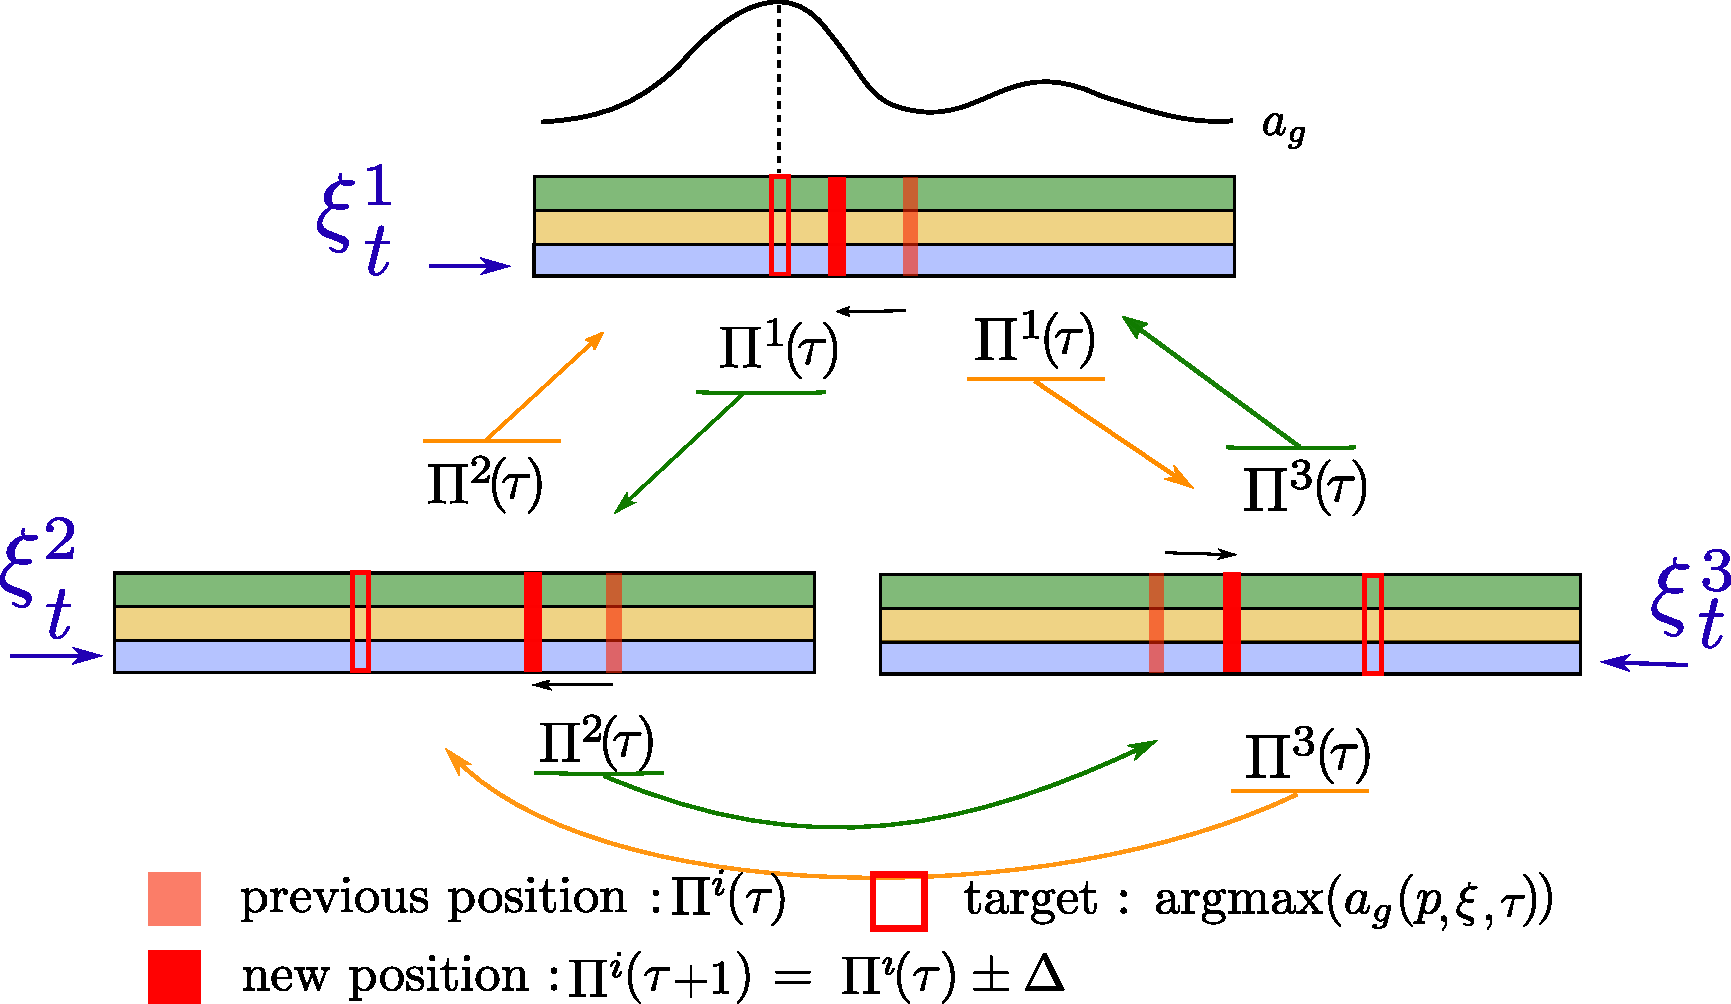
\includegraphics[width=0.6\textwidth]{relaxation.pdf}
\label{fig:relax}
\caption{description d'une étape de la relaxation dans l'architecture, aboutissant à un consensus entre cartes. Au sein d'une même itération $t$, les position des BMU $\bmu$ sont légèrement déplacées jusqu'à ce que toutes les positions $\bmu$ des cartes de l'architecture soient stable. Ces positions maximisent collectivement les activités globales de chaque carte. }
\end{figure}

\begin{figure}
\centering
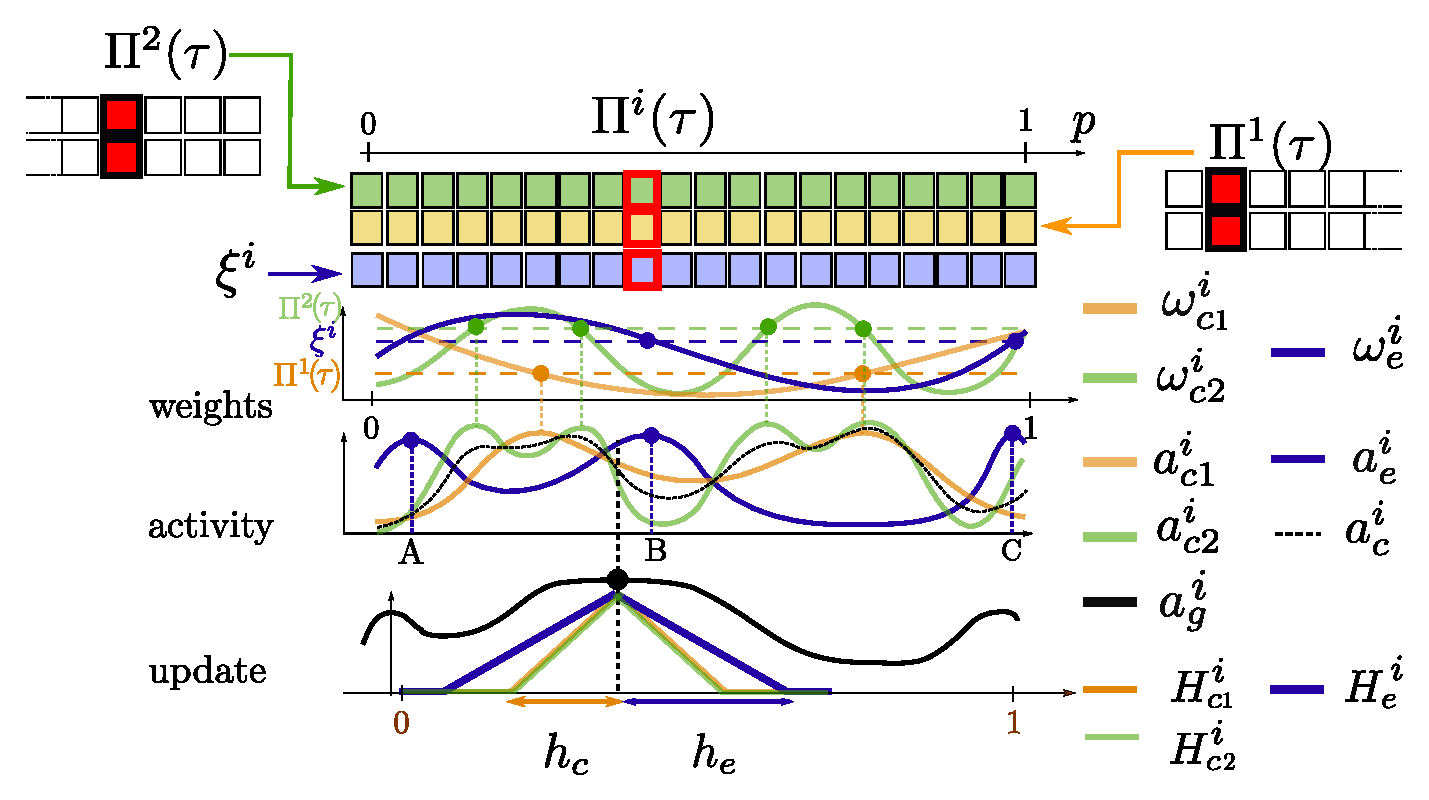
\includegraphics[width=0.8\textwidth]{one_map.pdf}
\caption{Description d'une carte au sein d'une architecture CxSOM. La carte recoit deux connexions de cartes voisines, et possède donc deux couches contextuelles}
\label{fig:one_map}
\end{figure}

\subsection{Mise à jour des poids}

Les poids sont mis à jour par rapport à leurs entrées respectives suivant l'équation \ref{eq:update}. Le BMU d'une carte est ainsi commun à toutes les couches. Les rayons de voisinage $h_e$ et $h_c$ ont des valeurs différentes ; celles-ci seront détaillée en partie suivante. 

\subsection{Résumé : Algorithme général}





